\documentclass[
	a4paper,
	oneside,
	BCOR = 10mm,
	DIV = 12,
	12pt,
	headings = normal,
]{scrartcl}

%%% Length calculations
\usepackage{calc}
%%%

%%% Support for color
\usepackage{xcolor}
\definecolor{lightblue}{HTML}{03A9F4}
\definecolor{red}{HTML}{F44336}
%%%

%%% Including graphics
\usepackage{graphicx}
%%%

%%% Font selection
\usepackage{fontspec}

\setromanfont{STIX Two Text}[
	SmallCapsFeatures = {LetterSpace = 8},
]

\setsansfont{IBM Plex Sans}[
	Scale = MatchUppercase,
]

\setmonofont{IBM Plex Mono}[
	Scale = MatchUppercase,
]
%%%

%%% Math typesetting
\usepackage{amsmath}

\usepackage{unicode-math}
\setmathfont{STIX Two Math}

\usepackage{IEEEtrantools}
%%%

%%% List settings
\usepackage{enumitem}
\setlist[enumerate]{%
	label*      = {\arabic*.},
	leftmargin  = *,
	labelindent = \parindent,
	topsep      = 1\baselineskip,
	parsep      = 0\baselineskip,
	itemsep     = 1\baselineskip,
	noitemsep, % override itemsep
}

\setlist[itemize]{%
	label*      = {—},
	leftmargin  = *,
	labelindent = \parindent,
	topsep      = 1\baselineskip,
	parsep      = 0\baselineskip,
	itemsep     = 1\baselineskip,
	noitemsep, % override itemsep
}

\setlist[description]{%
	font        = {\rmfamily\upshape\bfseries},
	topsep      = 1\baselineskip,
	parsep      = 0\baselineskip,
	itemsep     = 0\baselineskip,
}

%%%

%%% Structural elements typesetting
\setkomafont{pagenumber}{\rmfamily\upshape}
\setkomafont{disposition}{\rmfamily\bfseries}

% Sectioning
\RedeclareSectionCommand[
	beforeskip = -1\baselineskip,
	afterskip  = 1\baselineskip,
	font       = {\normalsize\bfseries\scshape},
]{section}

\RedeclareSectionCommand[
	beforeskip = -1\baselineskip,
	afterskip  = 1\baselineskip,
	font       = {\normalsize\bfseries\itshape},
]{subsection}

\RedeclareSectionCommand[
	beforeskip = -1\baselineskip,
	afterskip  = 1\baselineskip,
	font       = {\normalsize\bfseries},
]{subsubsection}

\RedeclareSectionCommand[
	beforeskip = -1\baselineskip,
	afterskip  = -0.5em,
	font       = {\normalsize\mdseries\scshape\addfontfeatures{Letters = {UppercaseSmallCaps}}},
]{paragraph}
%%%

%%% Typographic enhancements
\usepackage{microtype}
%%%

%%% Language-specific settings
\usepackage{polyglossia}
\setmainlanguage{ukrainian}
\setotherlanguages{english}
%%%

%%% Captions
\usepackage{caption}
\usepackage{subcaption}

%\DeclareCaptionLabelFormat{closing}{#2)}
%\captionsetup[subtable]{labelformat = closing}

%\captionsetup[subfigure]{labelformat = closing}

\captionsetup[table]{%
	aboveskip = 0\baselineskip,
	belowskip = 0\baselineskip,
}

\captionsetup[figure]{%
	aboveskip = 1\baselineskip,
	belowskip = 0\baselineskip,
}

\captionsetup[subfigure]{%
	labelformat = simple,
	labelformat = brace,
}
%%%

%%% Hyphenated ragged typesetting
\usepackage{ragged2e}
%%%

%%% Table typesetting
\usepackage{booktabs}
\usepackage{longtable}

\usepackage{multirow}

\usepackage{array}
\newcolumntype{v}[1]{>{\RaggedRight\arraybackslash\hspace{0pt}}p{#1}}
\newcolumntype{b}[1]{>{\Centering\arraybackslash\hspace{0pt}}p{#1}}
\newcolumntype{n}[1]{>{\RaggedLeft\arraybackslash\hspace{0pt}}p{#1}}
%%%

%%% Drawing
\usepackage{tikz}
\usepackage{tikzscale}
\usetikzlibrary{arrows.meta} % Stealth arrow tips
\usetikzlibrary{calc} % Coordinate calculations
\usetikzlibrary{positioning}
\usetikzlibrary{shapes.geometric} % Stealth arrow tips
%%%

%%% SI units typesetting
\usepackage{siunitx}
\sisetup{%
	output-decimal-marker = {,},
	exponent-product      = {\cdot},
	inter-unit-product    = \ensuremath{{} \cdot {}},
	per-mode              = symbol,
}
%%%

%%% Framing code listings
\usepackage{tcolorbox}
\tcbuselibrary{breakable}
\tcbuselibrary{minted}
\tcbuselibrary{skins}

\newtcblisting[
	auto counter,
	list inside,
	number within = section,
]{listingpython}[3][]{%
	minted language = python,
	minted style    = bw,
	minted options  = {%
		linenos,
		tabsize = 4,
		breaklines,
		% breakanywhere,
		fontsize = \footnotesize,
		autogobble
	},
	%
	% empty,
	sharp corners,
	colframe         = black,
	colback          = black!0,
	leftrule         = 0em,
	rightrule        = 0em,
	toprule          = 1pt, % orig = 0pt
	bottomrule       = 1pt, % orig = 0pt
	titlerule        = 0.5pt,
	colbacktitle     = black!0,
	coltitle         = black,
	toptitle         = 0.3em,
	bottomtitle      = 0.1em,
	borderline north = {1pt}{0pt}{black},
	borderline south = {1pt}{0pt}{black},
	before skip      = \intextsep,
	after  skip      = \intextsep,
	title            = {Лістинг \thetcbcounter: #2},
	list entry       = {\protect\numberline{\thetcbcounter}#2},
	left = 0em,
	right = 0em,
	%
	listing only,
	breakable,
	%
	label = {#3},
	%
	#1
}

\newtcbinputlisting[auto counter, list inside, number within = section]{\inputpython}[4][]{%
	minted language = python,
	minted style    = bw,
	minted options  = {%
		linenos,
		tabsize = 4,
		breaklines,
		breakbytokenanywhere,
		fontsize = \footnotesize,
	},
	%
	% empty,
	sharp corners,
	colframe         = black,
	colback          = black!0,
	leftrule         = 0em,
	rightrule        = 0em,
	toprule          = 0pt, % orig = 0pt
	bottomrule       = 0pt, % orig = 0pt
	titlerule        = 0.5pt,
	colbacktitle     = black!0,
	coltitle         = black,
	toptitle         = 0.3em,
	bottomtitle      = 0.1em,
	borderline north = {1pt}{0pt}{black},
	borderline south = {1pt}{0pt}{black},
	before skip      = \intextsep,
	after  skip      = \intextsep,
	title            = {Лістинг \thetcbcounter: #3},
	list entry       = {\protect\numberline{\thetcbcounter}#3},
	left = 0em,
	right = 0em,
	%
	listing file={#2},
	listing only,
	breakable,
	%
	label = {#4},
	%
	#1
}

% Customize minted
\usepackage{minted}
\setmintedinline{%
	style = bw,
	breaklines,
}

% Customize minted line numbers
\renewcommand{\theFancyVerbLine}{\ttfamily\scriptsize\arabic{FancyVerbLine}}

%%%

%%% Sideways table
\usepackage{pdflscape}
%%%

%%% Wrap text after sideways table
\usepackage{afterpage}
%%%

%%% Links and hyperreferences
\usepackage{hyperref}
\hypersetup{%
	bookmarksnumbered = true,
	colorlinks      = false,
	linkbordercolor = red,
	urlbordercolor  = lightblue,
	pdfborderstyle  = {/S/U/W 1.5},
}
%%%

%%% Length adjustments
% Set baselineskip, default is 14.5 pt
\linespread{1.068966} % ~15.5 pt
\setlength{\emergencystretch}{1em}
\setlength{\parindent}{1.5em}
\newlength{\gridunitwidth}
\setlength{\gridunitwidth}{\textwidth / 12}
%%%

%%% Custom commands
\newcommand{\allcaps}[1]{{\addfontfeatures{LetterSpace = 8, Kerning = Off}#1}}
\newcommand{\filename}[1]{\texttt{#1}}
\newcommand{\progname}[1]{\texttt{#1}}
\newcommand{\modulename}[1]{\texttt{#1}}
%%%

%%% Custom math commands
\newcommand{\longvar}[1]{\mathit{#1}}
%%%

\begin{document}

\begin{titlepage}
		\begin{center}
			Міністерство освіти і~науки України\\
			Національний авіаційний університет\\
			Навчально-науковий інститут комп'\-ютерних інформаційних технологій\\
			Кафедра комп'\-ютеризованих систем управління

			\vspace{\fill}
				Лабораторна робота №4\\
				з~дисципліни «Комп'\-ютерні системи»\\
				на~тему «Знаходження оптимальної модифікації обчислювальної системи для~обчислення арифметичних виразів»\\
				Варіант~№3

			\vspace{\fill}

			\begin{flushright}
				Виконав:\\
				студент \allcaps{ННІКІТ}\\
				групи СП-325\\
				Клокун В.\,Д.\\
				Перевірив:\\
				Ковальов М.\,О.
			\end{flushright}

			Київ 2019
		\end{center}
	\end{titlepage}

	\section{Мета роботи}
		Розробка ефективної структури обчислювальної системи для~обчислення арифметичних виразів.

	\section{Загальні теоретичні відомості}
		Критерії ефективності ОС. Як критерії ефективності розв'язання задачі (обчислення арифметичних виразів) будемо розглядати:
		\begin{enumerate}
			\item Коефіцієнт прискорення:
				\begin{IEEEeqnarray}{rCl}
					K_{\text{П}} = \frac{T_{0}}{T_{N}},
				\end{IEEEeqnarray}
				де $T_0$~— час розв’язання задачі в традиційній ЕОМ (однопроцесорній), який дорівнює сумі часу виконання операцій додавання, множення та ділення, які складають обчислювальну задачу, що розглядається; $T_{N}$~— час розв’язання задачі в ОС.
			\item Коефіцієнт завантаження процесорів (процесорних елементів)
				\begin{IEEEeqnarray}{rCl}
					K_{\text{З}} = \frac{T_{0}}{N \cdot T_{N}},
				\end{IEEEeqnarray}
			де $N$~— кількість процесорів (процесорних елементів) в ОС.
		\end{enumerate}

		Для визначення перерахованих показників ефективності достатньо знати не абсолютні величини часу виконання різних арифметичних операцій, а їх відносні співвідношення. Для цього введемо такі позначення:
		\begin{IEEEeqnarray}{rCl}
			\alpha = \frac{t_{\times}}{t_{+}}, \quad
			\beta  = \frac{t_{\div}}{t_{+}},
		\end{IEEEeqnarray}
		де $t_{+}$~— час виконання операції додавання, $t_{\times}$~— час виконання операції множення, $t_{\div}$~— час виконання операції ділення.

		\textit{Приклад.} Значну частину програм розв’язання інженерних і науково-технічних задач складають обчислення арифметичних виразів. Будь-який арифметичний вираз із змінними можна графічно подати у вигляді дерева. Дерево виразу складається з набору вузлів (вершин), кожний з яких містить окрім даних покажчики на вузли нижнього рівня. Верхній вузол (корінь дерева) відповідає операції, яка виконується останньою. З нього починається побудова дерева.
		На рис. 11 зображено дерево арифметичного виразу:
		\begin{IEEEeqnarray}{rCl}
			a + b \times c + d \div (e + f) + g \times h.
		\end{IEEEeqnarray}
		Час обчислення даного арифметичного виразу в традиційній ЕОМ можна визначити таким чином:
		\begin{IEEEeqnarray}{rCl}
			T_{0} = 4t_{+} + 2t_{\times} + t_{\div}.
		\end{IEEEeqnarray}

		Розглянемо можливість скорочення часу обчислення арифметичного виразу (11) за рахунок організації паралельного виконання операцій і використання обчислювальних систем різних структур.

		На рис. 12 дерево арифметичного виразу (11) у вигляді, зручному для паралельної обробки. Обчислення виразу (11) здійснюється за чотири етапи:
		\begin{enumerate}

			\item На першому етапі можливе паралельне виконання трьох операцій:
				\begin{IEEEeqnarray*}{rCl}
					O_1 = b \times c, \quad O_2 = e + f, \quad O_3 = g \times h.
				\end{IEEEeqnarray*}
			\item На другому етапі можливе паралельне виконання двох операцій:
				\begin{IEEEeqnarray*}{rCl}
					O_4 = a + O_1, \quad O_5 = d \div O_2.
				\end{IEEEeqnarray*}
			\item На третьому етапі можливе паралельне виконання однієї операції:
				\begin{IEEEeqnarray*}{rCl}
					O_6 = O_4 + O_5.
				\end{IEEEeqnarray*}
			\item На четвертому етапі виконується операція:
				\begin{IEEEeqnarray*}{rCl}
					O_7 = O_6 + O_3.
				\end{IEEEeqnarray*}
		\end{enumerate}

		Ранг задачі обчислення арифметичного виразу (11), який визначається кількістю виконуваних паралельно на кожному етапі операцій, змінюється від трьох на першому етапі до однієї на четвертому.

		Розглянемо організацію обчислення арифметичного виразу (11) в різних обчислювальних системах для випадку $N = 3$, $\alpha = 3$, $\beta = 3$.

		Час розв’язання задачі, що розглядається в традиційній ЕОМ при даних $\alpha$ і $\beta$, складе на основі формули (12) $T_0 = 11 t_{+}$.

		Для варіанта М2.1 є можливість організації паралельного виконання всіх трьох операцій на етапі 1 (рис. 4.2.).

		На рис. 4.2. зображені часові діаграми завантаженості процесорів системи.

		При такому розподілі операцій по процесорах час розв’язання задачі $T_{\text{M2.1}} = t_{\div} + 2 t_{+} = 6 t_{+}$.

		За рахунок зміни порядку виконання операцій при обчисленні арифметичних виразів можливе скорочення часу їх обчислення. Тобто знаходження більш оптимального алгоритму. Така оптимізація базується на тому, що деякі операції та операнди починаються певними законами, враховуючи які, можна здійснювати перетворення початкового виразу. Можна виділити такі закони, як комутативний, асоціативний, дистрибутивний та ін.

		\begin{figure}[!htbp]
			\centering
			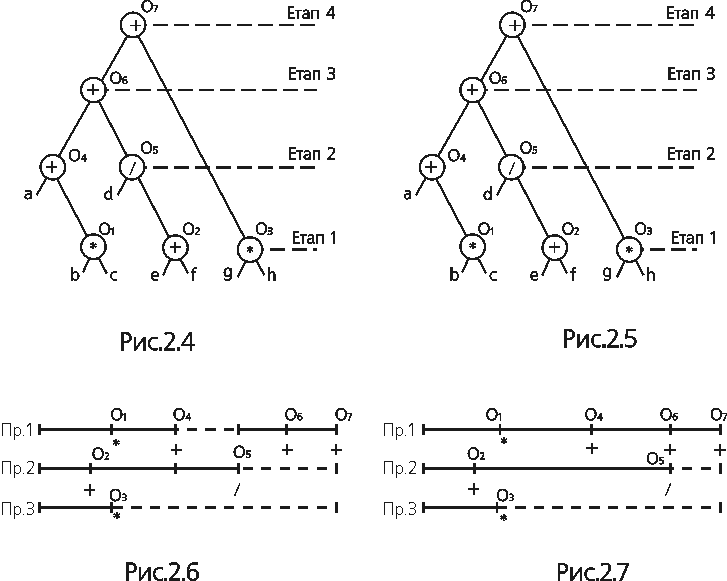
\includegraphics[height = 18\baselineskip]{./assets/01.png}
			\caption{Дерева арифметичних виразів та відповідні часові діаграми}
			\label{fig:expr-trees-time-diags}
		\end{figure}

		На рис.~\ref{fig:expr-trees-time-diags} показано змінене дерево арифметичного виразу (11).

		Як видно із часових діаграм роботи процесорів (рис.~\ref{fig:expr-trees-time-diags}), у цьому випадку можна скоротити час розв’язання задачі за рахунок ліквідації простою першого  процесора:
		\begin{IEEEeqnarray*}{rCl}
			T_{\text{M2.1}} = t_{\times} + 3t_{+} = 5 t_{+}.
		\end{IEEEeqnarray*}

	Використовуючи співвідношення (11) і (12) для прийнятих $N$, $\alpha$ i $\beta$, визначимо коефіцієнти прискорення і завантаження:
	\begin{IEEEeqnarray*}{rCl}
		K_{\text{П}} &=& \frac{T_0}{T_{\text{M2.1}}} = \num{2.2},\\[2\jot]
		K_{\text{З}} &=& \frac{T_0}{N \cdot T_{\text{M2.1}}} = \num{0.73}
	\end{IEEEeqnarray*}

		Для другого варіанта організації роботи системи (М2.2) характерне використання “вектор-інструкції”. При цьому необхідно враховувати, що час виконання кожної “вектор-інструкції” ($t_{\text{ві}}$) визначається часом виконання самої тривалої команди в цій “вектор-інструкції”.

		Послідовність і компоненти “вектор-інструкції” для реалізації в обчислювальних системах типу М2.2. арифметичного виразу, зображеного деревом на рис.~\ref{fig:expr-trees-time-diags} подані в табл.~\ref{tab:vector-instructions}.
		\begin{table}[!htbp]
			\centering
			\caption{Вектор-інструкції для реалізації арифметичного виразу в ОС типу М2.2}
			\label{tab:vector-instructions}
			\begin{tabular}{%
				v{3\gridunitwidth - 2\tabcolsep}
				v{3\gridunitwidth - 2\tabcolsep}
				v{3\gridunitwidth - 2\tabcolsep}
				v{3\gridunitwidth - 2\tabcolsep}
			}
				\toprule
					\multicolumn{3}{c}{Вектор-інструкція}\\
					\cmidrule(lr){1-3}
					Процесор 1 & Процесор 2 & Процесор 3 & $t_{\text{ві}}$ \\
				\midrule
					$O_1 = b \times c$ & $O_2 = e + f$ & $O_3 = g + h$ & $t_{\times}$ \\
					$O_4 = a + O_1$ & $O_5 = d \div O_2$ & & $t_{\div}$\\
					$O_6 = O_4 + O_3$ &  &  & $t_{+}$\\
					$O_7 = O_6 + O_5$ &  &  & $t_{+}$\\
				\bottomrule
			\end{tabular}
		\end{table}

		Часові діаграми завантаження процесорів системи показано на рис.~\ref{fig:cpu-load-diag}.
		\begin{figure}[!htbp]
			\centering
			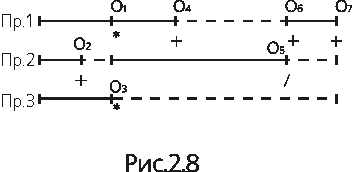
\includegraphics[height = 6\baselineskip]{./assets/02.png}
			\caption{Часова діаграма завантаження процесорів системи}
			\label{fig:cpu-load-diag}
		\end{figure}

		Значення коефіцієнтів прискорення і завантаження:
		\begin{IEEEeqnarray*}{rCl}
			K_{\text{П}} &=& \frac{T_0}{T_{\text{M2.2}}} = \num{1.6},\\[2\jot]
			K_{\text{З}} &=& \frac{T_0}{N \cdot T_{\text{M2.2}}} = \num{0.54}
		\end{IEEEeqnarray*}

		Обчислювальна система типу М3 в кожний момент часу допускає лише виконання однакових операцій. Тому доцільно звести дерево вихідного арифметичного виразу до вигляду, зручного для обробки в обчислювальній системі типу М3 (рис. 16). Обчислення арифметичного виразу, який розглядається в обчислювальній системі типу М3, здійснюється в п’ять етапів.

		При цьому:
		\begin{IEEEeqnarray*}{rCl}
			T_{M3} = t_{\times} + t_{\div} + 3t_{+} = 8 t_{+}.
		\end{IEEEeqnarray*}

		На рис.~\ref{fig:expr-tree-space-time-diag} зображена просторово-часова діаграма розв’язання задачі. Як видно, ранг задачі не перевищує 2 і один процесор при $N = 3$ не буде працювати. Пунктиром на просторово-часовій діаграмі позначена площа, що відповідає роботі, яку можна виконати на обчислювальній системі з $N = 3$ за час $T_{M3}$ , заштрихована площа просторово-часової діаграми відповідає роботі, виконаній системою в дійсності. Їх відношення і визначає коефіцієнт завантаження процесорів. Для розглянутої задачі $K_{\text{П}} = \num{1.37}$;  $K_{\text{З}} = \num{0.46}$.

		\begin{figure}[!htbp]
			\centering
			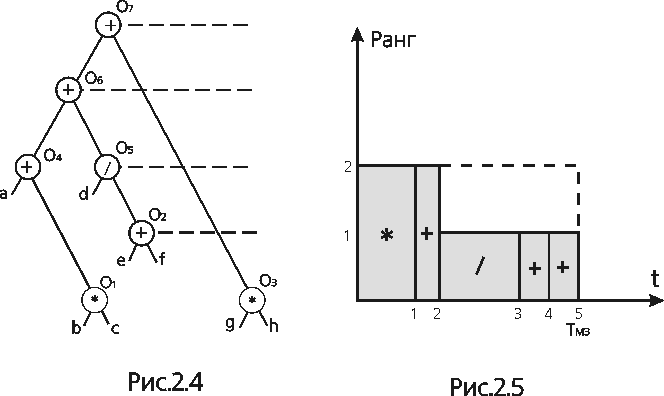
\includegraphics[height=8\baselineskip]{./assets/03.png}
			\caption{Дерево виразу та просторово-часова діаграма розв'язання задачі на~обчислювальній системі типу~M3}
			\label{fig:expr-tree-space-time-diag}
		\end{figure}

		В табл. 7 наведено значення коефіцієнтів прискорення і завантаження під час розв’язання задачі обчислення арифметичного виразу (11) в різних обчислювальних системах.

		\begin{table}[!htbp]
			\centering
			\caption{}
			\label{tab:speedup-load-coeffs}
			\begin{tabular}{
				v{2\gridunitwidth - 2\tabcolsep}
				n{2\gridunitwidth - 2\tabcolsep}
				n{2\gridunitwidth - 2\tabcolsep}
			}
				\toprule
					Тип ОС & $K_{\text{П}}$ & $K_{\text{З}}$ \\
				\midrule
					M2.1   & \num{2.20}     & \num{0.73}\\
					M2.2   & \num{1.60}     & \num{0.54}\\
					M3     & \num{1.37}     & \num{0.46}\\
				\bottomrule
			\end{tabular}
		\end{table}

		Значення коефіцієнтів прискорення і завантаження під час розв’язання задачі обчислення арифметичного виразу в різних ОС.

		Аналіз результатів ефективності різних структур обчислювальної системи під час розв’язання задачі, що розглядається, дозволяє зробити такі висновки:

		\begin{enumerate}
			\item Використання обчислювальної системи типу М2.1 дозволяє розв’язати задачу за мінімальний час.
			\item За ступенем використання обладнання (завантаження процесорів) перевагу слід віддати системі типу М2.1.
		\end{enumerate}

	\section{Хід роботи}
		Вихідними даними для лабораторної роботи є~арифметичний вираз:
		\begin{IEEEeqnarray}{rCl}
			\label{eq:task}
			(A + B) \mathbin{/} (C + D \cdot E) + F + (G + H) \mathbin{/} K \cdot L.
		\end{IEEEeqnarray}
		Також дана кількість процесорів~$N = 3$, значення коефіцієнта швидкості виконання множення~$\alpha = t_{\times} \mathbin{/} t_{+} = 2$  і~коефіцієнта швидкості виконання ділення~$\beta = t_{\div} \mathbin{/} t_{+} = 4$. Типи систем: M2.1, M3.

		Оскільки у виразі~\eqref{eq:task} виконується 5~операцій додавання, 2~операції множення і~2~операції ділення, то~час обчислення на~послідовній ЕОМ~$t_{0}$ обчислюється так: $t_{0} = 5t_{+} + 2t_{\times} + 2t_{\div}$. Так як~час виконання множення $t_{\times} = \alpha t_{+} = 2 t_{+}$ і~час виконання ділення $t_{\div} = \beta t_{+} = 4 t_{+}$, то час обчислення на послідовній ЕОМ~$T_{0}$ обчислюється так:
		\begin{IEEEeqnarray*}{rCl}
			T_{0} = 5t_{+} + 2t_{\times} + 2t_{\div} = 5t_{+} + 2 \cdot \alpha t_{+} + 2 \cdot \beta t_{+} = 5t_{+} + 2 \cdot 2 t_{+} + 2 \cdot 4t_{+} = 17t_{+}.
		\end{IEEEeqnarray*}

		% \subsection{Розрахунок критеріїв ефективності обчислювальних систем}
			\subsection{Обчислювальна система типу~M2.1 при кількості процесорів~$N = 3$}
			Система типу~M2.1 з~кількістю процесорів~$N = 3$ накладає такі обмеження:
			\begin{enumerate}
				\item Якщо кількість процесорів~$N = 3$, то на одному ярусі може бути не більше 3~операцій.
			\end{enumerate}
			Складаємо дерево арифметичного виразу~\eqref{eq:task}~(рис.~\ref{fig:expr-tree-m2p1-n3}).

			\begin{figure}[!htbp]
				\centering
				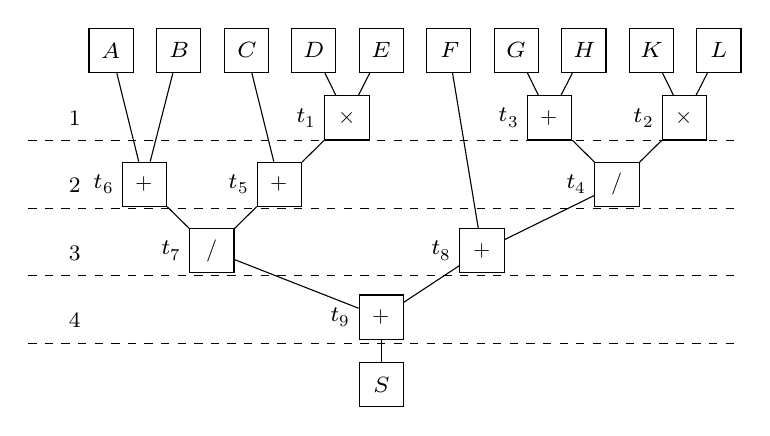
\begin{tikzpicture}[]
				\footnotesize
					\tikzset{main node/.style={draw,minimum size=2em}}
					\tikzset{every label/.style={label position=left}}
					\node[main node] (l05-a) {$A$};
					\node[main node, right = 1em of l05-a] (l05-b) {$B$};
					\node[main node, right = 1em of l05-b] (l05-c) {$C$};
					\node[main node, right = 1em of l05-c] (l05-d) {$D$};
					\node[main node, right = 1em of l05-d] (l05-e) {$E$};
					\node[main node, right = 1em of l05-e] (l05-f) {$F$};
					\node[main node, right = 1em of l05-f] (l05-g) {$G$};
					\node[main node, right = 1em of l05-g] (l05-h) {$H$};
					\node[main node, right = 1em of l05-h] (l05-k) {$K$};
					\node[main node, right = 1em of l05-k] (l05-l) {$L$};

					\begin{scope}[every node/.style = {anchor=north west}]
						\node[main node, label={$t_1$}, below right = 1em and 1.5em of l05-d.south west]  (l04-mul) {$\times$};
						\node[main node, label={$t_3$}, below right = 1em and 1.5em of l05-g.south west]  (l04-plus2) {$+$};
						\node[main node, label={$t_2$}, below right = 1em and 1.5em of l05-k.south west]  (l04-mul2) {$\times$};

						\node[main node, label={$t_6$}, below right = 4em and 1.5em of l05-a.south west]  (l03-plus2) {$+$};
						\node[main node, label={$t_5$}, below right = 4em and 1.5em of l05-c.south west]  (l03-plus) {$+$};
						\node[main node, label={$t_4$}, below right = 4em and 1.5em of l05-h.south west]  (l03-div) {$/$};

						\node[main node, label={$t_7$}, below right = 7em and 1.5em of l05-b.south west] (l02-div) {$/$};
						\node[main node, label={$t_8$}, below right = 7em and 1.5em of l05-f.south west] (l02-plus) {$+$};

						\node[main node, label={$t_9$}, below right  = 10em and 0em of l05-e.south west] (root-plus) {$+$};

						\node[main node, below right = 1em and 0 em of root-plus.south west] (root-S) {$S$};
					\end{scope}

					\begin{scope}
						\path[draw]
						(root-S)    edge node {} (root-plus)
						(root-plus) edge node {} (l02-div)
												edge node {} (l02-plus)
						(l02-div)   edge node {} (l03-plus)
												edge node {} (l03-plus2)
						(l02-plus)  edge node {} (l03-div)
												edge node {} (l05-f)
						(l03-plus)  edge node {} (l04-mul)
												edge node {} (l05-c)
						(l03-div)   edge node {} (l04-mul2)
												edge node {} (l04-plus2)
						(l03-plus2) edge node {} (l05-a)
												edge node {} (l05-b)
						(l04-mul)   edge node {} (l05-d)
												edge node {} (l05-e)
						(l04-plus2) edge node {} (l05-g)
												edge node {} (l05-h)
						(l04-mul2)  edge node {} (l05-k)
												edge node {} (l05-l)
						;
					\end{scope}

						%\path[dashed] (current bounding box.west) -- (current bounding box.east);
					\begin{scope}
						\node [minimum size = 2em, anchor = north east, below left = 1em and 0em of l05-a.south west] (l04) {Ярус 1};
						\node [minimum size = 2em, below = 1em of l04.south] (l03) {Ярус 2};
						\node [minimum size = 2em, below = 1em of l03.south] (l02) {Ярус 3};
						\node [minimum size = 2em, below = 1em of l02.south] (l01) {Ярус 4};

						\draw [dashed] (l04.south west) -- (l04.south west -| l05-l.east);
						\draw [dashed] (l03.south west) -- (l03.south west -| l05-l.east);
						\draw [dashed] (l02.south west) -- (l02.south west -| l05-l.east);
						\draw [dashed] (l01.south west) -- (l01.south west -| l05-l.east);
					\end{scope}
				\end{tikzpicture}
				\caption{Дерево арифметичного виразу $(A + B) \mathbin{/} (C + D \cdot E) + F + (G + H) \mathbin{/} K \cdot L$ для~обчислювальної системи типу~M2.1 при~кількості процесорів~$N = 3$}
				\label{fig:expr-tree-m2p1-n3}
			\end{figure}

			За деревом виразу підбираємо розташування операцій та складаємо часову діаграму~(рис.~\ref{fig:time-diag-cpu-usage-m2p1-n3}).

			\begin{figure}[!htbp]
				\centering
				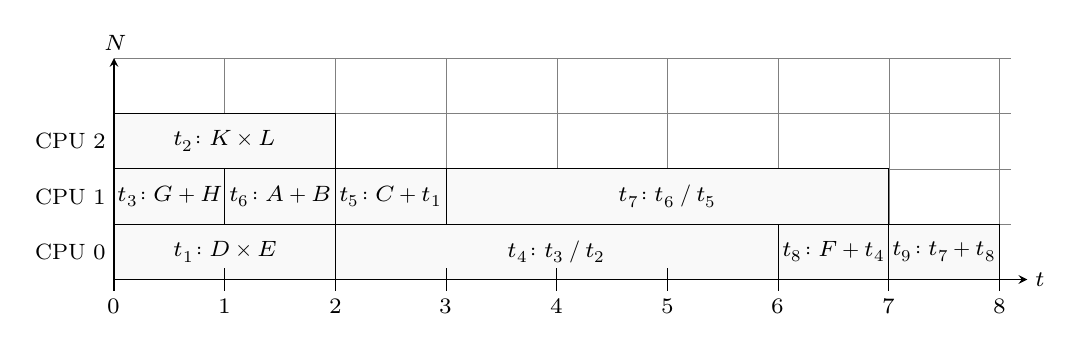
\begin{tikzpicture}[x = 4em, y = 2em]
					\footnotesize
					\draw[help lines, step=1] (0.0, 0.0) grid (8.1, 4.0);

					% Coordinate lines
					\begin{scope}[>=stealth]
						\draw[->] (0, 0) -- (8.25, 0) node[right] {$t$};
						\draw[->] (0, 0) -- (0, 4)   node[above] {$N$};
					\end{scope}

					\begin{scope}
						% t1
						\draw [fill = black!2.5] (0,0) rectangle node {$t_1\colon D \times E$} (2,1);
						% t3
						\draw [fill = black!2.5] (0,1) rectangle node {$t_3\colon G + H$} (1,2);
						% t2
						\draw [fill = black!2.5] (0,2) rectangle node {$t_2\colon K \times L$} (2,3);
						% t6
						\draw [fill = black!2.5] (1,1) rectangle node {$t_6\colon A + B$} (2,2);
						% t4
						\draw [fill = black!2.5] (2,0) rectangle node {$t_4\colon t_3 \mathbin{/} t_2$} (6,1);
						% t5
						\draw [fill = black!2.5] (2,1) rectangle node {$t_5\colon C + t_1$} (3,2);
						% t7
						\draw [fill = black!2.5] (3,1) rectangle node {$t_7\colon t_6 \mathbin{/} t_5$} (7,2);
						% t8
						\draw [fill = black!2.5] (6,0) rectangle node {$t_8\colon F + t_4$} (7,1);
						% t9
						\draw [fill = black!2.5] (7,0) rectangle node {$t_9\colon t_7 + t_8$} (8,1);
					\end{scope}

					\newcommand*{\TickSize}{0.5em}
					% x ticks
					\begin{scope}
						\foreach \x in {0,...,8} {%
								\draw ($(\x,0) + (0,-\TickSize)$) -- ($(\x,0) + (0,\TickSize)$)
										node [anchor = north, below = 1em] {$\x$};
						}
					\end{scope}
					% y ticks
					% \begin{scope}
					% 	\foreach \y in {0,...,3} {%
					% 			\draw ($(0,\y) + (-\TickSize,0)$) -- ($(0,\y) + (\TickSize,0)$)
					% 					node [anchor = east, left = 1em] {CPU $\y$};
					% 	}
					% \end{scope}

					\begin{scope}
						\foreach \y in {0,...,2} {%
							\node[anchor = east] at (0, \y + 0.5) {CPU $\y$};
						}
					\end{scope}
				\end{tikzpicture}
				\caption{Часова діаграма завантаженості процесорів системи типу~M2.1 при~кількості процесорів~$N = 3$}
				\label{fig:time-diag-cpu-usage-m2p1-n3}
			\end{figure}

			Як видно на осі~$Ot$, найдовший відрізок $\text{CPU}~0$ займає~8 одиниць, тобто виконання обчислення займає~$T_{M2.1} = 8t_{+}$.

			Обчисливши тривалість виконання обчислення на обчислювальній системі типу M2.1 з кількістю процесорів~$N = 3$, обчислюємо її критерії ефективності: коефіцієнт прискорення~$K_{\text{П}}$ і~коефіцієнт завантаження~$K_{\text{З}}$. Вони обчислюються так:
			\begin{IEEEeqnarray*}{rCl}
				K_{\text{П}} = \frac{T_0}{T_{M2.1}} = \frac{17 t_{+}}{8 t_{+}} = \num{2.125}, \quad
				K_{\text{З}} = \frac{T_0}{N \cdot T_{M2.1}} = \frac{17 t_{+}}{3 \cdot 8 t_{+}} = \num{0.71}.
			\end{IEEEeqnarray*}


			\subsection{Обчислювальна система типу~M3 при кількості процесорів~$N = 3$}
			Система типу~M3 з~кількістю процесорів~$N = 3$ накладає такі обмеження:
				\begin{enumerate}
					\item Якщо кількість процесорів~$N = 3$, то на одному ярусі може бути не більше 3~операцій.
					\item Так як використовується матрична обчислювальна система (тип M3), то на одному ярусі можуть виконуватись лише однакові операції.
				\end{enumerate}
				Складаємо дерево арифметичного виразу~\eqref{eq:task}~(рис.~\ref{fig:expr-tree-m3-n3}).

				\begin{figure}[!htbp]
					\centering
					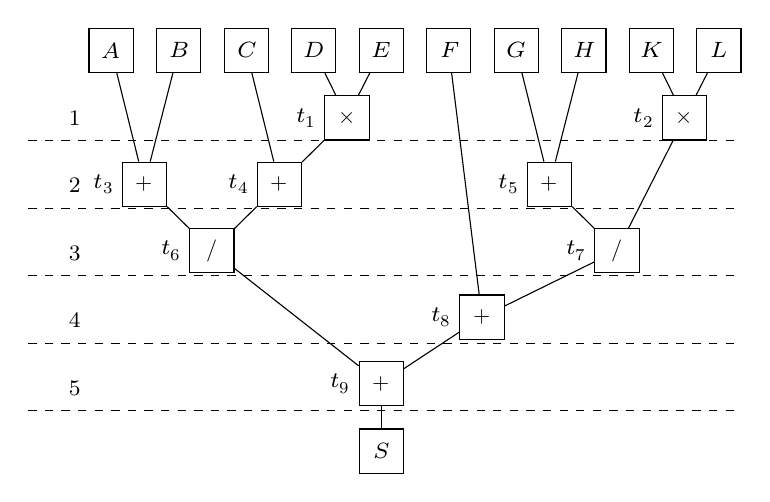
\begin{tikzpicture}[]
						\footnotesize
						\tikzset{main node/.style={draw,minimum size=2em}}
						\tikzset{every label/.style={label position=left}}
						\node[main node] (l05-a) {$A$};
						\node[main node, right = 1em of l05-a] (l05-b) {$B$};
						\node[main node, right = 1em of l05-b] (l05-c) {$C$};
						\node[main node, right = 1em of l05-c] (l05-d) {$D$};
						\node[main node, right = 1em of l05-d] (l05-e) {$E$};
						\node[main node, right = 1em of l05-e] (l05-f) {$F$};
						\node[main node, right = 1em of l05-f] (l05-g) {$G$};
						\node[main node, right = 1em of l05-g] (l05-h) {$H$};
						\node[main node, right = 1em of l05-h] (l05-k) {$K$};
						\node[main node, right = 1em of l05-k] (l05-l) {$L$};

						\begin{scope}[every node/.style = {anchor=north west}]
							% Layer 01
							\node[main node, label={$t_1$}, below right = 1em and 1.5em of l05-d.south west]  (l04-mul) {$\times$};
							\node[main node, label={$t_2$}, below right = 1em and 1.5em of l05-k.south west]  (l04-mul2) {$\times$};

							% Layer 02
							\node[main node, label={$t_3$}, below right = 4em and 1.5em of l05-a.south west]  (l03-plus2) {$+$};
							\node[main node, label={$t_4$}, below right = 4em and 1.5em of l05-c.south west]  (l03-plus) {$+$};
							\node[main node, label={$t_5$}, below right = 4em and 1.5em of l05-g.south west]  (l04-plus2) {$+$};

							% Layer 03
							\node[main node, label={$t_6$}, below right = 7em and 1.5em of l05-b.south west] (l02-div) {$/$};
							\node[main node, label={$t_7$}, below right = 7em and 1.5em of l05-h.south west]  (l03-div) {$/$};

							% Layer 04
							\node[main node, label={$t_8$}, below right = 10em and 1.5em of l05-f.south west] (l02-plus) {$+$};

							% Layer 05
							\node[main node, label={$t_9$}, below right  = 13em and 0em of l05-e.south west] (root-plus) {$+$};

							% Root
							\node[main node, below right = 1em and 0 em of root-plus.south west] (root-S) {$S$};
						\end{scope}

						\begin{scope}
							\path[draw]
							(root-S)    edge node {} (root-plus)
							(root-plus) edge node {} (l02-div)
													edge node {} (l02-plus)
							(l02-div)   edge node {} (l03-plus)
													edge node {} (l03-plus2)
							(l02-plus)  edge node {} (l03-div)
													edge node {} (l05-f)
							(l03-plus)  edge node {} (l04-mul)
													edge node {} (l05-c)
							(l03-div)   edge node {} (l04-mul2)
													edge node {} (l04-plus2)
							(l03-plus2) edge node {} (l05-a)
													edge node {} (l05-b)
							(l04-mul)   edge node {} (l05-d)
													edge node {} (l05-e)
							(l04-plus2) edge node {} (l05-g)
													edge node {} (l05-h)
							(l04-mul2)  edge node {} (l05-k)
													edge node {} (l05-l)
							;
						\end{scope}

							%\path[dashed] (current bounding box.west) -- (current bounding box.east);
						\begin{scope}
							\node [minimum size = 2em, anchor = north east, below left = 1em and 0em of l05-a.south west] (l04) {Ярус 1};
							\node [minimum size = 2em, below = 1em of l04.south] (l03) {Ярус 2};
							\node [minimum size = 2em, below = 1em of l03.south] (l02) {Ярус 3};
							\node [minimum size = 2em, below = 1em of l02.south] (l01) {Ярус 4};
							\node [minimum size = 2em, below = 1em of l01.south] (l00) {Ярус 5};

							\draw [dashed] (l04.south west) -- (l04.south west -| l05-l.east);
							\draw [dashed] (l03.south west) -- (l03.south west -| l05-l.east);
							\draw [dashed] (l02.south west) -- (l02.south west -| l05-l.east);
							\draw [dashed] (l01.south west) -- (l01.south west -| l05-l.east);
							\draw [dashed] (l00.south west) -- (l00.south west -| l05-l.east);
						\end{scope}

					\end{tikzpicture}
					\caption{Дерево арифметичного виразу $(A + B) \mathbin{/} (C + D \cdot E) + F + (G + H) \mathbin{/} K \cdot L$ для~обчислювальної системи типу~M3 при~кількості процесорів~$N = 3$}
					\label{fig:expr-tree-m3-n3}
				\end{figure}

				За деревом виразу підбираємо розташування операцій та складаємо часову діаграму~(рис.~\ref{fig:time-diag-cpu-usage-m3-n3}).

				\begin{figure}[!htbp]
					\centering
					{\scriptsize
					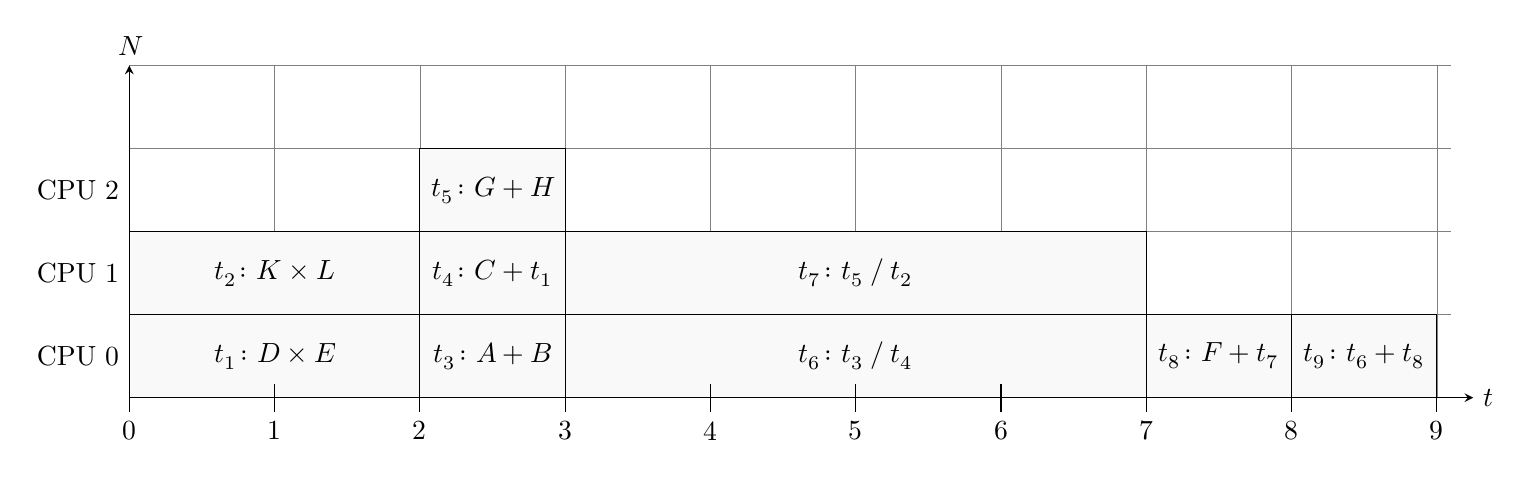
\begin{tikzpicture}[x = 5.25em, y = 3em]
						\draw[help lines, step=1] (0.0, 0.0) grid (9.1, 4.0);

						% Coordinate lines
						\begin{scope}[>=stealth]
							\draw[->] (0, 0) -- (9.25, 0) node[right] {$t$};
							\draw[->] (0, 0) -- (0, 4)   node[above] {$N$};
						\end{scope}

						\begin{scope}
							% t1
							\draw [fill = black!2.5] (0,0) rectangle node {$t_1\colon D \times E$} (2,1);
							% t2
							\draw [fill = black!2.5] (0,1) rectangle node {$t_2\colon K \times L$} (2,2);
							% t3
							\draw [fill = black!2.5] (2,0) rectangle node {$t_3\colon A + B$} (3,1);
							% t4
							\draw [fill = black!2.5] (2,1) rectangle node {$t_4\colon C + t_1$} (3,2);
							% t5
							\draw [fill = black!2.5] (2,2) rectangle node {$t_5\colon G + H$} (3,3);
							% t6
							\draw [fill = black!2.5] (3,0) rectangle node {$t_6\colon t_3 \mathbin{/} t_4$} (7,1);
							% t7
							\draw [fill = black!2.5] (3,1) rectangle node {$t_7\colon t_5 \mathbin{/} t_2$} (7,2);
							% t8
							\draw [fill = black!2.5] (7,0) rectangle node {$t_8\colon F + t_7$} (8,1);
							% t9
							\draw [fill = black!2.5] (8,0) rectangle node {$t_9\colon t_6 + t_8$} (9,1);
						\end{scope}

						\newcommand*{\TickSize}{0.5em}
						% x ticks
						\begin{scope}
							\foreach \x in {0,...,9} {%
									\draw ($(\x,0) + (0,-\TickSize)$) -- ($(\x,0) + (0,\TickSize)$)
											node [anchor = north, below = 1em] {$\x$};
							}
						\end{scope}
						% y ticks
						% \begin{scope}
						% 	\foreach \y in {0,...,3} {%
						% 			\draw ($(0,\y) + (-\TickSize,0)$) -- ($(0,\y) + (\TickSize,0)$)
						% 					node [anchor = east, left = 1em] {CPU $\y$};
						% 	}
						% \end{scope}

						\begin{scope}
							\foreach \y in {0,...,2} {%
								\node[anchor = east] at (0, \y + 0.5) {CPU $\y$};
							}
						\end{scope}
					\end{tikzpicture}
					}
					\caption{Часова діаграма завантаженості процесорів системи типу~M3 при~кількості процесорів~$N = 3$}
					\label{fig:time-diag-cpu-usage-m3-n3}
				\end{figure}

				Як видно на осі~$Ot$, найдовший відрізок $\text{CPU}~0$ займає 9~одиниць, тобто виконання обчислення займає~$T_{M3} = 9t_{+}$.

				Обчисливши тривалість виконання обчислення на обчислювальній системі типу M3 з кількістю процесорів~$N = 3$, обчислюємо її критерії ефективності: коефіцієнт прискорення~$K_{\text{П}}$ і~коефіцієнт завантаження~$K_{\text{З}}$. Вони обчислюються так:
				\begin{IEEEeqnarray*}{rCl}
					K_{\text{П}} = \frac{T_0}{T_{M3}} = \frac{17 t_{+}}{9 t_{+}} = \num{1.9}, \quad
					K_{\text{З}} = \frac{T_0}{N \cdot T_{M3}} = \frac{17 t_{+}}{3 \cdot 9 t_{+}} = \num{0.63}.
				\end{IEEEeqnarray*}

			\subsection{Обчислювальна система типу~M2.1 при кількості процесорів~$N = 2$}
				Система типу~M2.1 з~кількістю процесорів~$N = 3$ накладає такі обмеження:
					\begin{enumerate}
						\item Якщо кількість процесорів~$N = 2$, то на одному ярусі може бути не більше 2~операцій.
					\end{enumerate}
				Складаємо дерево арифметичного виразу~\eqref{eq:task}~(рис.~\ref{fig:expr-tree-m3-n2}).

				\begin{figure}[!htbp]
					\centering
					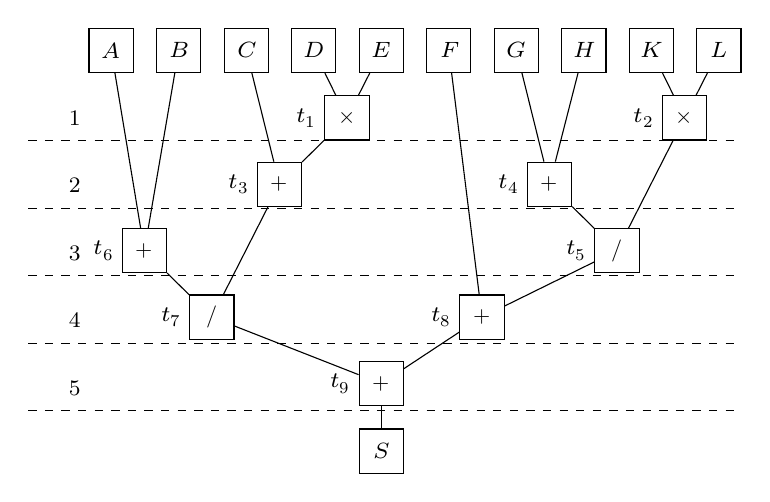
\begin{tikzpicture}[]
						\footnotesize
						\tikzset{main node/.style={draw,minimum size=2em}}
						\tikzset{every label/.style={label position=left}}
						\node[main node] (l05-a) {$A$};
						\node[main node, right = 1em of l05-a] (l05-b) {$B$};
						\node[main node, right = 1em of l05-b] (l05-c) {$C$};
						\node[main node, right = 1em of l05-c] (l05-d) {$D$};
						\node[main node, right = 1em of l05-d] (l05-e) {$E$};
						\node[main node, right = 1em of l05-e] (l05-f) {$F$};
						\node[main node, right = 1em of l05-f] (l05-g) {$G$};
						\node[main node, right = 1em of l05-g] (l05-h) {$H$};
						\node[main node, right = 1em of l05-h] (l05-k) {$K$};
						\node[main node, right = 1em of l05-k] (l05-l) {$L$};

						\begin{scope}[every node/.style = {anchor=north west}]
							% Layer 01
							\node[main node, label={$t_1$}, below right = 1em and 1.5em of l05-d.south west]  (l04-mul) {$\times$};
							\node[main node, label={$t_2$}, below right = 1em and 1.5em of l05-k.south west]  (l04-mul2) {$\times$};

							% Layer 02
							\node[main node, label={$t_3$}, below right = 4em and 1.5em of l05-c.south west]  (l03-plus) {$+$};
							\node[main node, label={$t_4$}, below right = 4em and 1.5em of l05-g.south west]  (l04-plus2) {$+$};

							% Layer 03
							\node[main node, label={$t_6$}, below right = 7em and 1.5em of l05-a.south west]  (l03-plus2) {$+$};
							\node[main node, label={$t_5$}, below right = 7em and 1.5em of l05-h.south west]  (l03-div) {$/$};

							% Layer 04
							\node[main node, label={$t_7$}, below right = 10em and 1.5em of l05-b.south west] (l02-div) {$/$};
							\node[main node, label={$t_8$}, below right = 10em and 1.5em of l05-f.south west] (l02-plus) {$+$};

							% Layer 05
							\node[main node, label={$t_9$}, below right  = 13em and 0em of l05-e.south west] (root-plus) {$+$};

							% Root
							\node[main node, below right = 1em and 0 em of root-plus.south west] (root-S) {$S$};
						\end{scope}

						\begin{scope}
							\path[draw]
							(root-S)    edge node {} (root-plus)
							(root-plus) edge node {} (l02-div)
													edge node {} (l02-plus)
							(l02-div)   edge node {} (l03-plus)
													edge node {} (l03-plus2)
							(l02-plus)  edge node {} (l03-div)
													edge node {} (l05-f)
							(l03-plus)  edge node {} (l04-mul)
													edge node {} (l05-c)
							(l03-div)   edge node {} (l04-mul2)
													edge node {} (l04-plus2)
							(l03-plus2) edge node {} (l05-a)
													edge node {} (l05-b)
							(l04-mul)   edge node {} (l05-d)
													edge node {} (l05-e)
							(l04-plus2) edge node {} (l05-g)
													edge node {} (l05-h)
							(l04-mul2)  edge node {} (l05-k)
													edge node {} (l05-l)
							;
						\end{scope}

							%\path[dashed] (current bounding box.west) -- (current bounding box.east);
						\begin{scope}
							\node [minimum size = 2em, anchor = north east, below left = 1em and 0em of l05-a.south west] (l04) {Ярус 1};
							\node [minimum size = 2em, below = 1em of l04.south] (l03) {Ярус 2};
							\node [minimum size = 2em, below = 1em of l03.south] (l02) {Ярус 3};
							\node [minimum size = 2em, below = 1em of l02.south] (l01) {Ярус 4};
							\node [minimum size = 2em, below = 1em of l01.south] (l00) {Ярус 5};

							\draw [dashed] (l04.south west) -- (l04.south west -| l05-l.east);
							\draw [dashed] (l03.south west) -- (l03.south west -| l05-l.east);
							\draw [dashed] (l02.south west) -- (l02.south west -| l05-l.east);
							\draw [dashed] (l01.south west) -- (l01.south west -| l05-l.east);
							\draw [dashed] (l00.south west) -- (l00.south west -| l05-l.east);
						\end{scope}

					\end{tikzpicture}
					\caption{Дерево арифметичного виразу $(A + B) \mathbin{/} (C + D \cdot E) + F + (G + H) \mathbin{/} K \cdot L$ для~обчислювальної системи типу~M2.1 при~кількості процесорів~$N = 2$}
					\label{fig:expr-tree-m2p1-n2}
				\end{figure}

				За деревом виразу підбираємо розташування операцій та складаємо часову діаграму~(рис.~\ref{fig:time-diag-cpu-usage-m2p1-n2}).

				\begin{figure}[!htbp]
					\centering
					{\scriptsize
					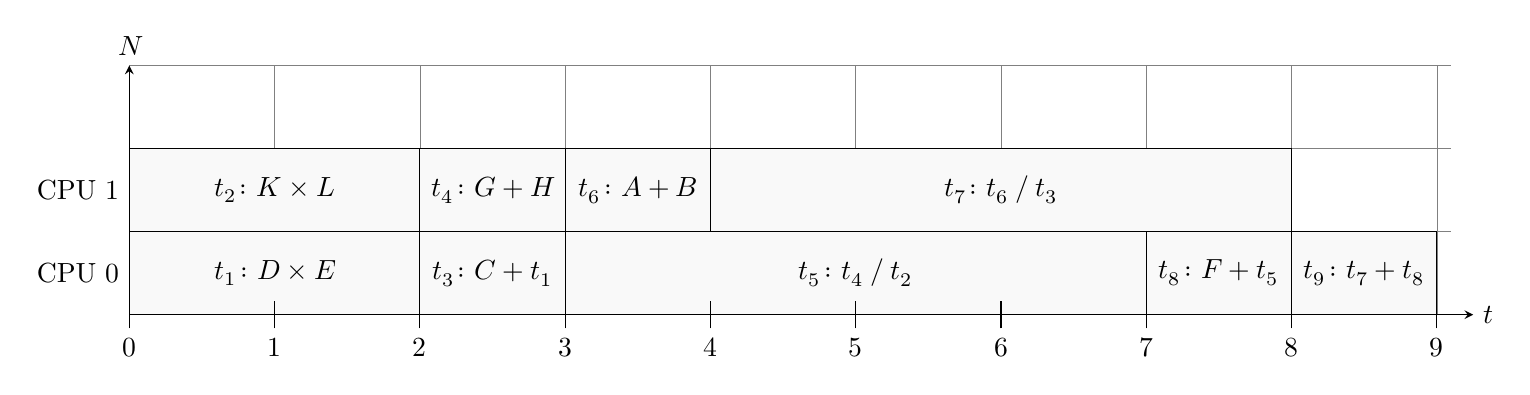
\begin{tikzpicture}[x = 5.25em, y = 3em]
						\draw[help lines, step=1] (0.0, 0.0) grid (9.1, 3.0);

						% Coordinate lines
						\begin{scope}[>=stealth]
							\draw[->] (0, 0) -- (9.25, 0) node[right] {$t$};
							\draw[->] (0, 0) -- (0, 3)   node[above] {$N$};
						\end{scope}

						\begin{scope}
							% t1
							\draw [fill = black!2.5] (0,0) rectangle node {$t_1\colon D \times E$} (2,1);
							% t2
							\draw [fill = black!2.5] (0,1) rectangle node {$t_2\colon K \times L$} (2,2);
							% t3
							\draw [fill = black!2.5] (2,0) rectangle node {$t_3\colon C + t_1$} (3,1);
							% t4
							\draw [fill = black!2.5] (2,1) rectangle node {$t_4\colon G + H$} (3,2);
							% t5
							\draw [fill = black!2.5] (3,0) rectangle node {$t_5\colon t_4 \mathbin{/} t_2$} (7,1);
							% t6
							\draw [fill = black!2.5] (3,1) rectangle node {$t_6\colon A + B$} (4,2);
							% t7
							\draw [fill = black!2.5] (4,1) rectangle node {$t_7\colon t_6 \mathbin{/} t_3$} (8,2);
							% t8
							\draw [fill = black!2.5] (7,0) rectangle node {$t_8\colon F + t_5$} (8,1);
							% t9
							\draw [fill = black!2.5] (8,0) rectangle node {$t_9\colon t_7 + t_8$} (9,1);
						\end{scope}

						\newcommand*{\TickSize}{0.5em}
						% x ticks
						\begin{scope}
							\foreach \x in {0,...,9} {%
									\draw ($(\x,0) + (0,-\TickSize)$) -- ($(\x,0) + (0,\TickSize)$)
											node [anchor = north, below = 1em] {$\x$};
							}
						\end{scope}
						% y ticks
						% \begin{scope}
						% 	\foreach \y in {0,...,3} {%
						% 			\draw ($(0,\y) + (-\TickSize,0)$) -- ($(0,\y) + (\TickSize,0)$)
						% 					node [anchor = east, left = 1em] {CPU $\y$};
						% 	}
						% \end{scope}

						\begin{scope}
							\foreach \y in {0,...,1} {%
								\node[anchor = east] at (0, \y + 0.5) {CPU $\y$};
							}
						\end{scope}
					\end{tikzpicture}
					}
					\caption{Часова діаграма завантаженості процесорів системи типу~M2.1 при~кількості процесорів~$N = 2$}
					\label{fig:time-diag-cpu-usage-m2p1-n2}
				\end{figure}

				Як видно на осі~$Ot$, найдовший відрізок $\text{CPU}~0$ займає 9~одиниць, тобто виконання обчислення займає~$T_{M3} = 9t_{+}$.

				Обчисливши тривалість виконання обчислення на обчислювальній системі типу M2.1 з кількістю процесорів~$N = 2$, обчислюємо її критерії ефективності: коефіцієнт прискорення~$K_{\text{П}}$ і~коефіцієнт завантаження~$K_{\text{З}}$. Вони обчислюються так:
				\begin{IEEEeqnarray*}{rCl}
					K_{\text{П}} = \frac{T_0}{T_{M3}} = \frac{17 t_{+}}{9 t_{+}} = \num{1.9}, \quad
					K_{\text{З}} = \frac{T_0}{N \cdot T_{M3}} = \frac{17 t_{+}}{2 \cdot 9 t_{+}} = \num{0.94}.
				\end{IEEEeqnarray*}

			\subsection{Обчислювальна система типу~M3 при кількості процесорів~$N = 2$}
				Система типу~M3 з~кількістю процесорів~$N = 3$ накладає такі обмеження:
				\begin{enumerate}
					\item Якщо кількість процесорів~$N = 2$, то на одному ярусі може бути не більше 2~операцій.
					\item Так як використовується матрична обчислювальна система (тип M3), то на одному ярусі можуть виконуватись лише однакові операції.
				\end{enumerate}
				Складаємо дерево арифметичного виразу~\eqref{eq:task}~(рис.~\ref{fig:expr-tree-m3-n2}).

				\begin{figure}[!htbp]
					\centering
					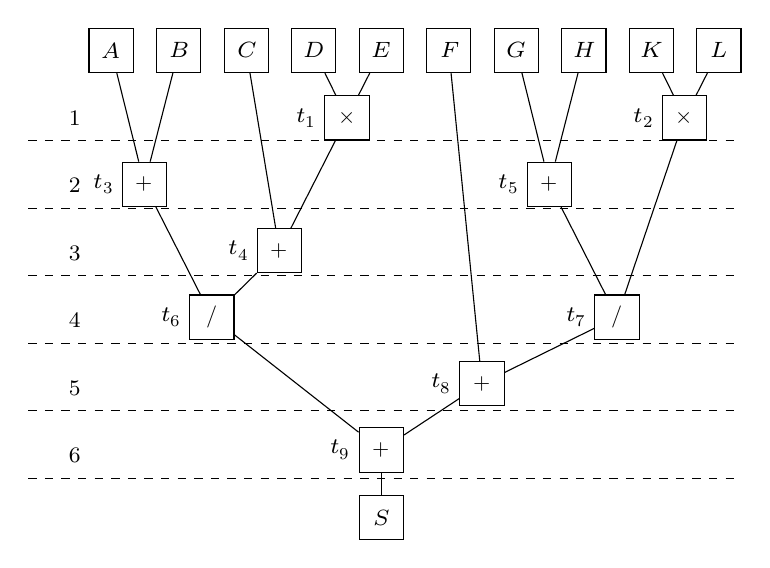
\begin{tikzpicture}[]
						\footnotesize
						\tikzset{main node/.style={draw,minimum size=2em}}
						\tikzset{every label/.style={label position=left}}
						\node[main node] (l05-a) {$A$};
						\node[main node, right = 1em of l05-a] (l05-b) {$B$};
						\node[main node, right = 1em of l05-b] (l05-c) {$C$};
						\node[main node, right = 1em of l05-c] (l05-d) {$D$};
						\node[main node, right = 1em of l05-d] (l05-e) {$E$};
						\node[main node, right = 1em of l05-e] (l05-f) {$F$};
						\node[main node, right = 1em of l05-f] (l05-g) {$G$};
						\node[main node, right = 1em of l05-g] (l05-h) {$H$};
						\node[main node, right = 1em of l05-h] (l05-k) {$K$};
						\node[main node, right = 1em of l05-k] (l05-l) {$L$};

						\begin{scope}[every node/.style = {anchor=north west}]
							% Layer 01
							\node[main node, label={$t_1$}, below right = 1em and 1.5em of l05-d.south west]  (l04-mul) {$\times$};
							\node[main node, label={$t_2$}, below right = 1em and 1.5em of l05-k.south west]  (l04-mul2) {$\times$};

							% Layer 02
							\node[main node, label={$t_3$}, below right = 4em and 1.5em of l05-a.south west]  (l03-plus2) {$+$};
							\node[main node, label={$t_5$}, below right = 4em and 1.5em of l05-g.south west]  (l04-plus2) {$+$};

							% Layer 03
							\node[main node, label={$t_4$}, below right = 7em and 1.5em of l05-c.south west]  (l03-plus) {$+$};

							% Layer 04
							\node[main node, label={$t_6$}, below right = 10em and 1.5em of l05-b.south west] (l02-div) {$/$};
							\node[main node, label={$t_7$}, below right = 10em and 1.5em of l05-h.south west]  (l03-div) {$/$};

							% Layer 05
							\node[main node, label={$t_8$}, below right = 13em and 1.5em of l05-f.south west] (l02-plus) {$+$};

							% Layer 06
							\node[main node, label={$t_9$}, below right  = 16em and 0em of l05-e.south west] (root-plus) {$+$};

							% Root
							\node[main node, below right = 1em and 0 em of root-plus.south west] (root-S) {$S$};
						\end{scope}

						\begin{scope}
							\path[draw]
							(root-S)    edge node {} (root-plus)
							(root-plus) edge node {} (l02-div)
													edge node {} (l02-plus)
							(l02-div)   edge node {} (l03-plus)
													edge node {} (l03-plus2)
							(l02-plus)  edge node {} (l03-div)
													edge node {} (l05-f)
							(l03-plus)  edge node {} (l04-mul)
													edge node {} (l05-c)
							(l03-div)   edge node {} (l04-mul2)
													edge node {} (l04-plus2)
							(l03-plus2) edge node {} (l05-a)
													edge node {} (l05-b)
							(l04-mul)   edge node {} (l05-d)
													edge node {} (l05-e)
							(l04-plus2) edge node {} (l05-g)
													edge node {} (l05-h)
							(l04-mul2)  edge node {} (l05-k)
													edge node {} (l05-l)
							;
						\end{scope}

							%\path[dashed] (current bounding box.west) -- (current bounding box.east);
						\begin{scope}
							\node [minimum size = 2em, anchor = north east, below left = 1em and 0em of l05-a.south west] (l04) {Ярус 1};
							\node [minimum size = 2em, below = 1em of l04.south] (l03) {Ярус 2};
							\node [minimum size = 2em, below = 1em of l03.south] (l02) {Ярус 3};
							\node [minimum size = 2em, below = 1em of l02.south] (l01) {Ярус 4};
							\node [minimum size = 2em, below = 1em of l01.south] (l00) {Ярус 5};
							\node [minimum size = 2em, below = 1em of l00.south] (lm1) {Ярус 6};

							\draw [dashed] (l04.south west) -- (l04.south west -| l05-l.east);
							\draw [dashed] (l03.south west) -- (l03.south west -| l05-l.east);
							\draw [dashed] (l02.south west) -- (l02.south west -| l05-l.east);
							\draw [dashed] (l01.south west) -- (l01.south west -| l05-l.east);
							\draw [dashed] (l00.south west) -- (l00.south west -| l05-l.east);
							\draw [dashed] (lm1.south west) -- (lm1.south west -| l05-l.east);
						\end{scope}

					\end{tikzpicture}
					\caption{Дерево арифметичного виразу $(A + B) \mathbin{/} (C + D \cdot E) + F + (G + H) \mathbin{/} K \cdot L$ для~обчислювальної системи типу~M3 при~кількості процесорів~$N = 2$}
					\label{fig:expr-tree-m3-n2}
				\end{figure}

				За деревом виразу підбираємо розташування операцій та складаємо часову діаграму~(рис.~\ref{fig:time-diag-cpu-usage-m3-n2}).

				\begin{figure}[!htbp]
					\centering
					{\scriptsize
					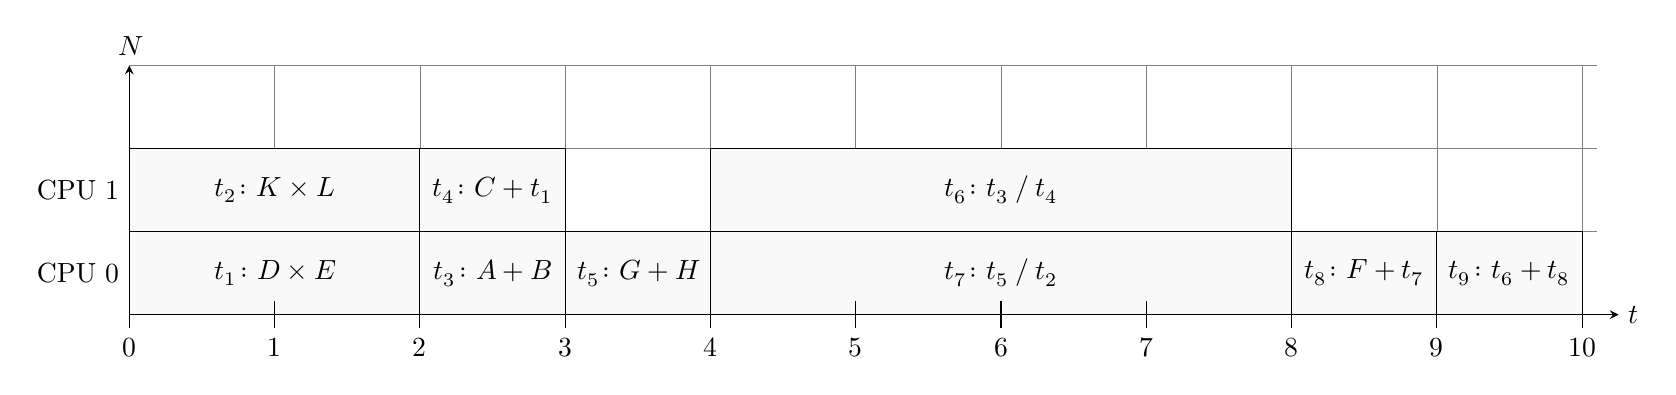
\begin{tikzpicture}[x = 5.25em, y = 3em]
						\draw[help lines, step=1] (0.0, 0.0) grid (10.1, 3.0);

						% Coordinate lines
						\begin{scope}[>=stealth]
							\draw[->] (0, 0) -- (10.25, 0) node[right] {$t$};
							\draw[->] (0, 0) -- (0, 3)   node[above] {$N$};
						\end{scope}

						\begin{scope}
							% t1
							\draw [fill = black!2.5] (0,0) rectangle node {$t_1\colon D \times E$} (2,1);
							% t2
							\draw [fill = black!2.5] (0,1) rectangle node {$t_2\colon K \times L$} (2,2);
							% t3
							\draw [fill = black!2.5] (2,0) rectangle node {$t_3\colon A + B$} (3,1);
							% t4
							\draw [fill = black!2.5] (2,1) rectangle node {$t_4\colon C + t_1$} (3,2);
							% t5
							\draw [fill = black!2.5] (3,0) rectangle node {$t_5\colon G + H$} (4,1);
							% t7
							\draw [fill = black!2.5] (4,0) rectangle node {$t_7\colon t_5 \mathbin{/} t_2$} (8,1);
							% t6
							\draw [fill = black!2.5] (4,1) rectangle node {$t_6\colon t_3 \mathbin{/} t_4$} (8,2);
							% t8
							\draw [fill = black!2.5] (8,0) rectangle node {$t_8\colon F + t_7$} (9,1);
							% t9
							\draw [fill = black!2.5] (9,0) rectangle node {$t_9\colon t_6 + t_8$} (10,1);
						\end{scope}

						\newcommand*{\TickSize}{0.5em}
						% x ticks
						\begin{scope}
							\foreach \x in {0,...,10} {%
									\draw ($(\x,0) + (0,-\TickSize)$) -- ($(\x,0) + (0,\TickSize)$)
											node [anchor = north, below = 1em] {$\x$};
							}
						\end{scope}
						% y ticks
						% \begin{scope}
						% 	\foreach \y in {0,...,3} {%
						% 			\draw ($(0,\y) + (-\TickSize,0)$) -- ($(0,\y) + (\TickSize,0)$)
						% 					node [anchor = east, left = 1em] {CPU $\y$};
						% 	}
						% \end{scope}

						\begin{scope}
							\foreach \y in {0,...,1} {%
								\node[anchor = east] at (0, \y + 0.5) {CPU $\y$};
							}
						\end{scope}
					\end{tikzpicture}
					}
					\caption{Часова діаграма завантаженості процесорів системи типу~M3 при~кількості процесорів~$N = 2$}
					\label{fig:time-diag-cpu-usage-m3-n2}
				\end{figure}

				Як видно на осі~$Ot$, найдовший відрізок $\text{CPU}~0$ займає 10~одиниць, тобто виконання обчислення займає~$T_{M3} = 10t_{+}$.

				Обчисливши тривалість виконання обчислення на обчислювальній системі типу M3 з кількістю процесорів~$N = 2$, обчислюємо її критерії ефективності: коефіцієнт прискорення~$K_{\text{П}}$ і~коефіцієнт завантаження~$K_{\text{З}}$. Вони обчислюються так:
				\begin{IEEEeqnarray*}{rCl}
					K_{\text{П}} = \frac{T_0}{T_{M3}} = \frac{17 t_{+}}{10 t_{+}} = \num{1.7}, \quad
					K_{\text{З}} = \frac{T_0}{N \cdot T_{M3}} = \frac{17 t_{+}}{2 \cdot 10 t_{+}} = \num{0.85}.
				\end{IEEEeqnarray*}

	\section{Висновок}
		Виконуючи дану лабораторну роботу, ми~розробили ефективну структуру обчислювальної системи для обчислення арифметичних виразів. Під час розробки структури ми визначили характеристики ефективності заданих обчислювальних систем~(табл.~\ref{tab:efficiency-comparison}).
		\begin{table}[!htbp]
			\centering
			\caption{Характеристики ефективності розглянутих обчислювальних систем}
			\label{tab:efficiency-comparison}
			\begin{tabular}{
				v{4\gridunitwidth - 2\tabcolsep}
				n{2\gridunitwidth - 2\tabcolsep}
				n{2\gridunitwidth - 2\tabcolsep}
				n{2\gridunitwidth - 2\tabcolsep}
				n{2\gridunitwidth - 2\tabcolsep}
			}
				\toprule
					Кількість процесорів & \multicolumn{2}{r}{$N = 3$} & \multicolumn{2}{r}{$N = 2$}\\
					\cmidrule(lr){2-3} \cmidrule(lr){4-5}
					Тип ОС & $K_{\text{П}}$ & $K_{\text{З}}$ & $K_{\text{П}}$ & $K_{\text{З}}$\\
				\midrule
				M2.1 & \num{2.125} & \num{0.71} & \num{1.9} & \num{0.94}\\
				M3   & \num{1.900} & \num{0.63} & \num{1.7} & \num{0.85}\\
				\bottomrule
			\end{tabular}
		\end{table}

		Визначені характеристики показують, що для обчислення заданого арифметичного виразу із заданими параметрами найбільше підходять обчислювальні системи типу M2.1, оскільки значення коефіцієнтів прискорення~$K_{\text{П}}$ і коефіцієнтів завантаження більші, ніж значення відповідних коефіцієнтів у системах типу M3.

		В залежності від потреб реалізації при виборі кількості процесорів для створення обчислювальної машини можна керуватись таким принципом: якщо реалізація повинна надавати максимальне прискорення, незважаючи на ціну, варто обрати кількість процесорів~$N = 3$; якщо ж реалізація повинна якнайбільш завантажувати існуючі процесори та коштувати менше, то варто реалізувати обчислювальну систему з кількістю процесорів~$N = 2$.

\end{document}

